\documentclass[conference]{IEEEtran}
\IEEEoverridecommandlockouts
% The preceding line is only needed to identify funding in the first footnote. If that is unneeded, please comment it out.
% \usepackage{cite}
\usepackage{amsmath,amssymb,amsfonts}
\usepackage{algorithmic}
\usepackage{graphicx}
\usepackage{textcomp}
\usepackage{xcolor}
\usepackage{url}
\usepackage{listings}
\usepackage{microtype}
\usepackage[numbers,compress]{natbib}
\usepackage{tabularx}
\def\BibTeX{{\rm B\kern-.05em{\sc i\kern-.025em b}\kern-.08em
    T\kern-.1667em\lower.7ex\hbox{E}\kern-.125emX}}
\begin{document}

\title{Hashiko\\
}

\author{\IEEEauthorblockN{Jackie Ma}
    \IEEEauthorblockA{\textit{Department of Computing} \\
        \textit{British Columbia Institute of Technology}\\
        Burnaby, Canada \\
        jma149@my.bcit.ca}
}

\maketitle

\begin{abstract}
Hashiko is a distributed monitoring system that tracks file integrity across multiple endpoints. Agents compute individual SHA-256 hashes for each monitored file and send reports to a central server over HTTPS. This agent-server design enables centralized monitoring across distributed systems. The server stores records and generates alerts when changes are detected. A web interface provides a timeline view of hash history, an alert panel and per-agent configuration management. The system focuses on accuracy, secure transfer and scalability. Automated tests cover the agent and server and run on every push through CI. Scope includes agents, server, storage and interface. Out of scope are malware analysis, snapshots and compliance reporting. Hashiko provides centralized visibility into file integrity across distributed systems.
\end{abstract}

\begin{IEEEkeywords}
    agents, alerts, central server, distributed monitoring, file integrity, per-file hashing, web interface
\end{IEEEkeywords}

\section*{List of Abbreviations}

\begin{tabularx}{\columnwidth}{@{}p{1.2cm}X@{}}
AIDE  & Advanced Intrusion Detection Environment \\
API   & Application Programming Interface \\
CI    & Continuous Integration \\
FIM   & File Integrity Monitoring \\
HIDS  & Host-based Intrusion Detection System \\
HTML  & HyperText Markup Language \\
HTTP  & HyperText Transfer Protocol \\
HTTPS & HyperText Transfer Protocol Secure \\
JSON  & JavaScript Object Notation \\
JSONB & JSON Binary (PostgreSQL data type) \\
OS    & Operating System \\
OSSEC & Open Source HIDS Security \\
SHA-256 & Secure Hash Algorithm 256-bit \\
SIEM  & Security Information and Event Management \\
SQL   & Structured Query Language \\
TLS   & Transport Layer Security \\
UI    & User Interface \\
\end{tabularx}

\section{Introduction}

Traditional file integrity monitors operate independently on each system. This creates management overhead in distributed environments. Attackers can disable local monitoring tools when they gain administrative access. Centralized monitoring addresses this vulnerability.

Hashiko is a distributed monitoring system that tracks file integrity across multiple endpoints. The project implements file integrity monitoring with centralized storage and queue-based retry logic for network resilience. Endpoint agents collect file hashes from critical system directories. All data is sent with timestamps to a central server for storage.

The goal is to provide centralized file integrity monitoring across distributed systems. Security teams can view hash changes from multiple endpoints in one interface.

\subsection{Endpoint Agents}

Endpoint agents are lightweight programs that run on each monitored system. They compute individual SHA-256 hashes for every file in each monitored directory and send timestamped reports to the central server. Volatile files and files above a configurable size threshold are skipped to reduce noise and prevent hangs on large directories. Each agent has a unique identity derived from the username, hostname and machine ID. On first run, the agent exchanges a one-time registration token for a persistent API key used to authenticate all subsequent requests.

\subsection{Centralized Server}

The server ingests, validates and stores hash reports from distributed agents. Built with Flask and PostgreSQL, the \texttt{/api/store} endpoint decodes JSON and inserts records with parameterized queries to prevent SQL injection. A composite index on timestamp and agent\_id enables fast queries. The \texttt{/api/hashes} endpoint returns all records with change detection applied. The \texttt{/api/config} endpoint serves watch paths and the file size threshold to agents. The \texttt{/api/register} endpoint handles one-time agent registration.

\subsection{Web Interface}

The web interface is built with vanilla HTML, CSS and JavaScript. Access is restricted behind a login page with session-based authentication. Once logged in, the agent grid shows all monitored machines with alert badges for recent changes. Clicking an agent shows the hash timeline, where each row represents a report. Rows with changes expand to list the exact files added, modified or deleted. A config panel allows the admin to set watch paths and the file size threshold per agent. An alert panel surfaces all changes detected in the last 24 hours.

\section{Problem Statement}

Organizations face increasing risks from both external attackers and insider threats. Traditional file integrity monitors operate independently on each system. This creates several problems. Local tools can be disabled by attackers with administrator privileges. Periodic checking creates detection delays. Higher inspection frequency improves detection but degrades performance. Manual policy configuration becomes impractical in distributed environments \cite{abdullah}.

User-space integrity checkers can only verify if files were modified between checking operations \cite{kaczmarek}. During this period, attackers can replace system files with backdoors or trojans \cite{kaczmarek}. Traditional FIM tools face a fundamental trade-off. High-frequency inspection maintains effectiveness but hurts performance. Low-frequency inspection reduces overhead but allows threats to persist undetected.

A centralized system that aggregates hash records from multiple endpoints can improve monitoring efficiency. Centralized monitoring is essential for security. Attackers with administrator privileges can compromise local security tools. Remote monitoring from a privileged server provides protection even when the monitored system is compromised \cite{abdullah}.

\begin{table}[h]
\centering
\caption{Challenges Addressed in This Project}
\begin{tabular}{|p{4cm}|p{4cm}|}
\hline
\textbf{Type of Challenge} & \textbf{Challenges} \\
\hline
Detection & Isolated event detection, local tool compromise \\
\hline
Performance & High-frequency inspection overhead \\
\hline
Operational & Manual policy configuration, distributed management \\
\hline
\end{tabular}
\end{table}

\section{Background}

The first source, Kaczmarek and Wrobel's Modern Approaches to File System Integrity Checking, addresses the challenges related to file integrity monitoring. The paper analyzed modern approaches to file system integrity checking, comparing user-space and kernel-space integrity checkers. Their review revealed trade-offs between periodic checking and real-time monitoring approaches. Among these, the technical challenges of detection delays and performance overhead \cite{kaczmarek} stood out. User-space integrity checkers can only verify if files were modified between checking operations, creating windows of vulnerability where compromised files may execute before detection \cite{kaczmarek}. Investigations are significantly impacted when temporal context is missing between security events \cite{kaczmarek}.

The second source, Abdullah et al.'s File Integrity Monitor Scheduling Based on File Security Level Classification, investigated file integrity monitor scheduling strategies. The paper emphasized that centralized monitoring is essential for security, as attackers with administrator privileges can compromise local security tools \cite{abdullah}. Remote monitoring from a privileged server provides protection even when the monitored system is compromised. Traditional file integrity checkers store baseline databases that are updated periodically, requiring significant maintenance overhead. Security tools need to correlate events across time when conducting investigations. For example, AIDE and Samhain schedule periodic checks at fixed intervals but cannot detect multi-step attacks spread over time. Similarly, OSSEC is designed for centralized logging but lacks real-time temporal chaining at the host level \cite{abdullah}.

In addition, commercial SIEM systems such as Splunk Enterprise Security and QRadar provide event correlation. However, they require enterprise infrastructure and specialized configuration. Systems like I3FS and SOFFIC achieve real-time monitoring but require kernel-level modifications that limit portability. Users are not able to deploy these systems across different platforms, causing slower adoption. These problems directly relate to this project. The goal is to provide centralized file integrity monitoring with simple deployment.

\section{Implementation}

\subsection{Prototype}

For the prototype, basic agent-server communication and file integrity monitoring were implemented. The agent was created in Go and hashes directories using SHA-256. Five critical directories are monitored: /boot, /usr/bin, /usr/sbin, /etc and /root. These directories contain common attack targets \cite{abdullah}. Volatile paths like .cache, .mozilla and tmp were filtered to reduce false positives. The agent generates JSON output including timestamp and directory hashes.

The backend server was created in Go using net/http and PostgreSQL. Routes were created for data ingest (\texttt{/api/store}) and viewing stored records. Data was transmitted via HTTP POST to the server. The server received agent data and inserted records with parameterized queries to prevent SQL injection.

A PostgreSQL database was set up with a hash\_records table storing timestamp, agent\_id and hash values for monitored directories. A composite index on (timestamp, agent\_id) was added to optimize queries.

\subsection{Milestone 1}

For Milestone 1, the backend was rewritten from Go to Python for simpler management. Composite indexes were added to improve query performance. PostgreSQL composite indexes on (timestamp, agent\_id) enable fast queries. These indexes significantly improve retrieval speed for queries involving multiple columns.

\subsection{Milestone 2}

For Milestone 2, a message queue mechanism was implemented. The queue system saves JSON hash data to local files when the server is unreachable. This prevents data loss during network interruptions. The implementation includes initialization of a queue directory, saving timestamped JSON files and a processing function that retries sending queued data to the server. Successfully transmitted files are then removed.

\subsection{Milestone 3}

For Milestone 3, hash comparison, alerts and login were implemented. The backend now compares each new report against the previous one for the same agent and flags any hash value that changed. An alert panel in the web UI surfaces changes detected in the last 24 hours. Agent cards are highlighted when alerts are active. All web UI routes were secured behind a login page with session-based authentication. Sessions expire after 24 hours of inactivity.

\subsection{Milestone 4}

For Milestone 4, agent identity, registration and security hardening were implemented. Each agent generates a unique ID in the format \texttt{user@hostname (machine-id)} using \texttt{/etc/machine-id}. A one-time registration token exchanges for a persistent API key saved to \texttt{/etc/hashiko/api\_key} with restricted file permissions. The agent enforces HTTPS on all API calls. The backend enforces SSL on database connections, sends an HSTS header and sets secure cookie flags. Admins can configure monitored paths per agent from the web UI. The backend was deployed on Render and the database on Supabase.

\subsection{Milestone 5}

For Milestone 5, per-file hashing, a file size threshold and automated testing were implemented. The \texttt{hashFiles} function replaces the previous directory-level approach. It walks each monitored directory and computes an individual SHA-256 hash for every file, returning a map of file path to hash value. Files above a configurable size threshold are skipped to prevent hangs on large media directories. The threshold is stored per agent in the database and adjustable from the web UI. The frontend was redesigned as a timeline where rows with changes expand to show the exact files affected. Automated tests were written for both the agent and backend. A GitHub Actions workflow runs all tests on every push.

\section{Complexity}

The project integrates distributed agents, HTTPS communication and PostgreSQL storage. The system must collect data from multiple endpoints reliably. Network failures must be handled without losing reports. This requires queue-based retry logic with file persistence.

The agent must efficiently hash large directory trees on a per-file basis. Volatile paths must be filtered to reduce false positives. Files above a configurable size threshold must be skipped to prevent performance issues on directories containing large media files. The server must validate incoming data and prevent SQL injection. Secure agent authentication requires a registration flow with token exchange and persistent key storage.

The JSONB schema must support arbitrary numbers of monitored file paths per agent without schema changes. Change detection must compare thousands of file hashes across consecutive reports efficiently. The web UI must render large numbers of file paths in a readable timeline format.

This project requires independent design decisions that go beyond coursework. Trade-offs between detection coverage and system performance must be evaluated.

\section{Methodology}

The project follows an agent-server design with a central database and web interface. This architecture separates data collection from storage. This pattern appears in centralized monitoring systems. Centralized management enables efficient monitoring of multiple systems. It addresses scalability limitations of standalone FIM tools.

Agents compute file hashes, monitor file paths and send timestamped events. The server ingests, validates and stores events. The web interface displays hash records in a timeline format.

\subsection{System Architecture}

Figure~\ref{fig:systems} shows the system architecture. Endpoints run Linux agents that compute per-file SHA-256 hashes across configurable monitored directories. Agents authenticate with a Bearer token and transmit hash reports via HTTPS POST to \texttt{/api/store}. The server validates and inserts records into PostgreSQL. A local queue stores failed transmissions for retry on the next run. The web interface requires login and fetches records from \texttt{/api/hashes}, displaying them in a timeline view with change detection and alerts. Figure~\ref{fig:sequence} shows the sequence of operations from agent registration through to the admin view.

\begin{figure}[h!]
    \centering
    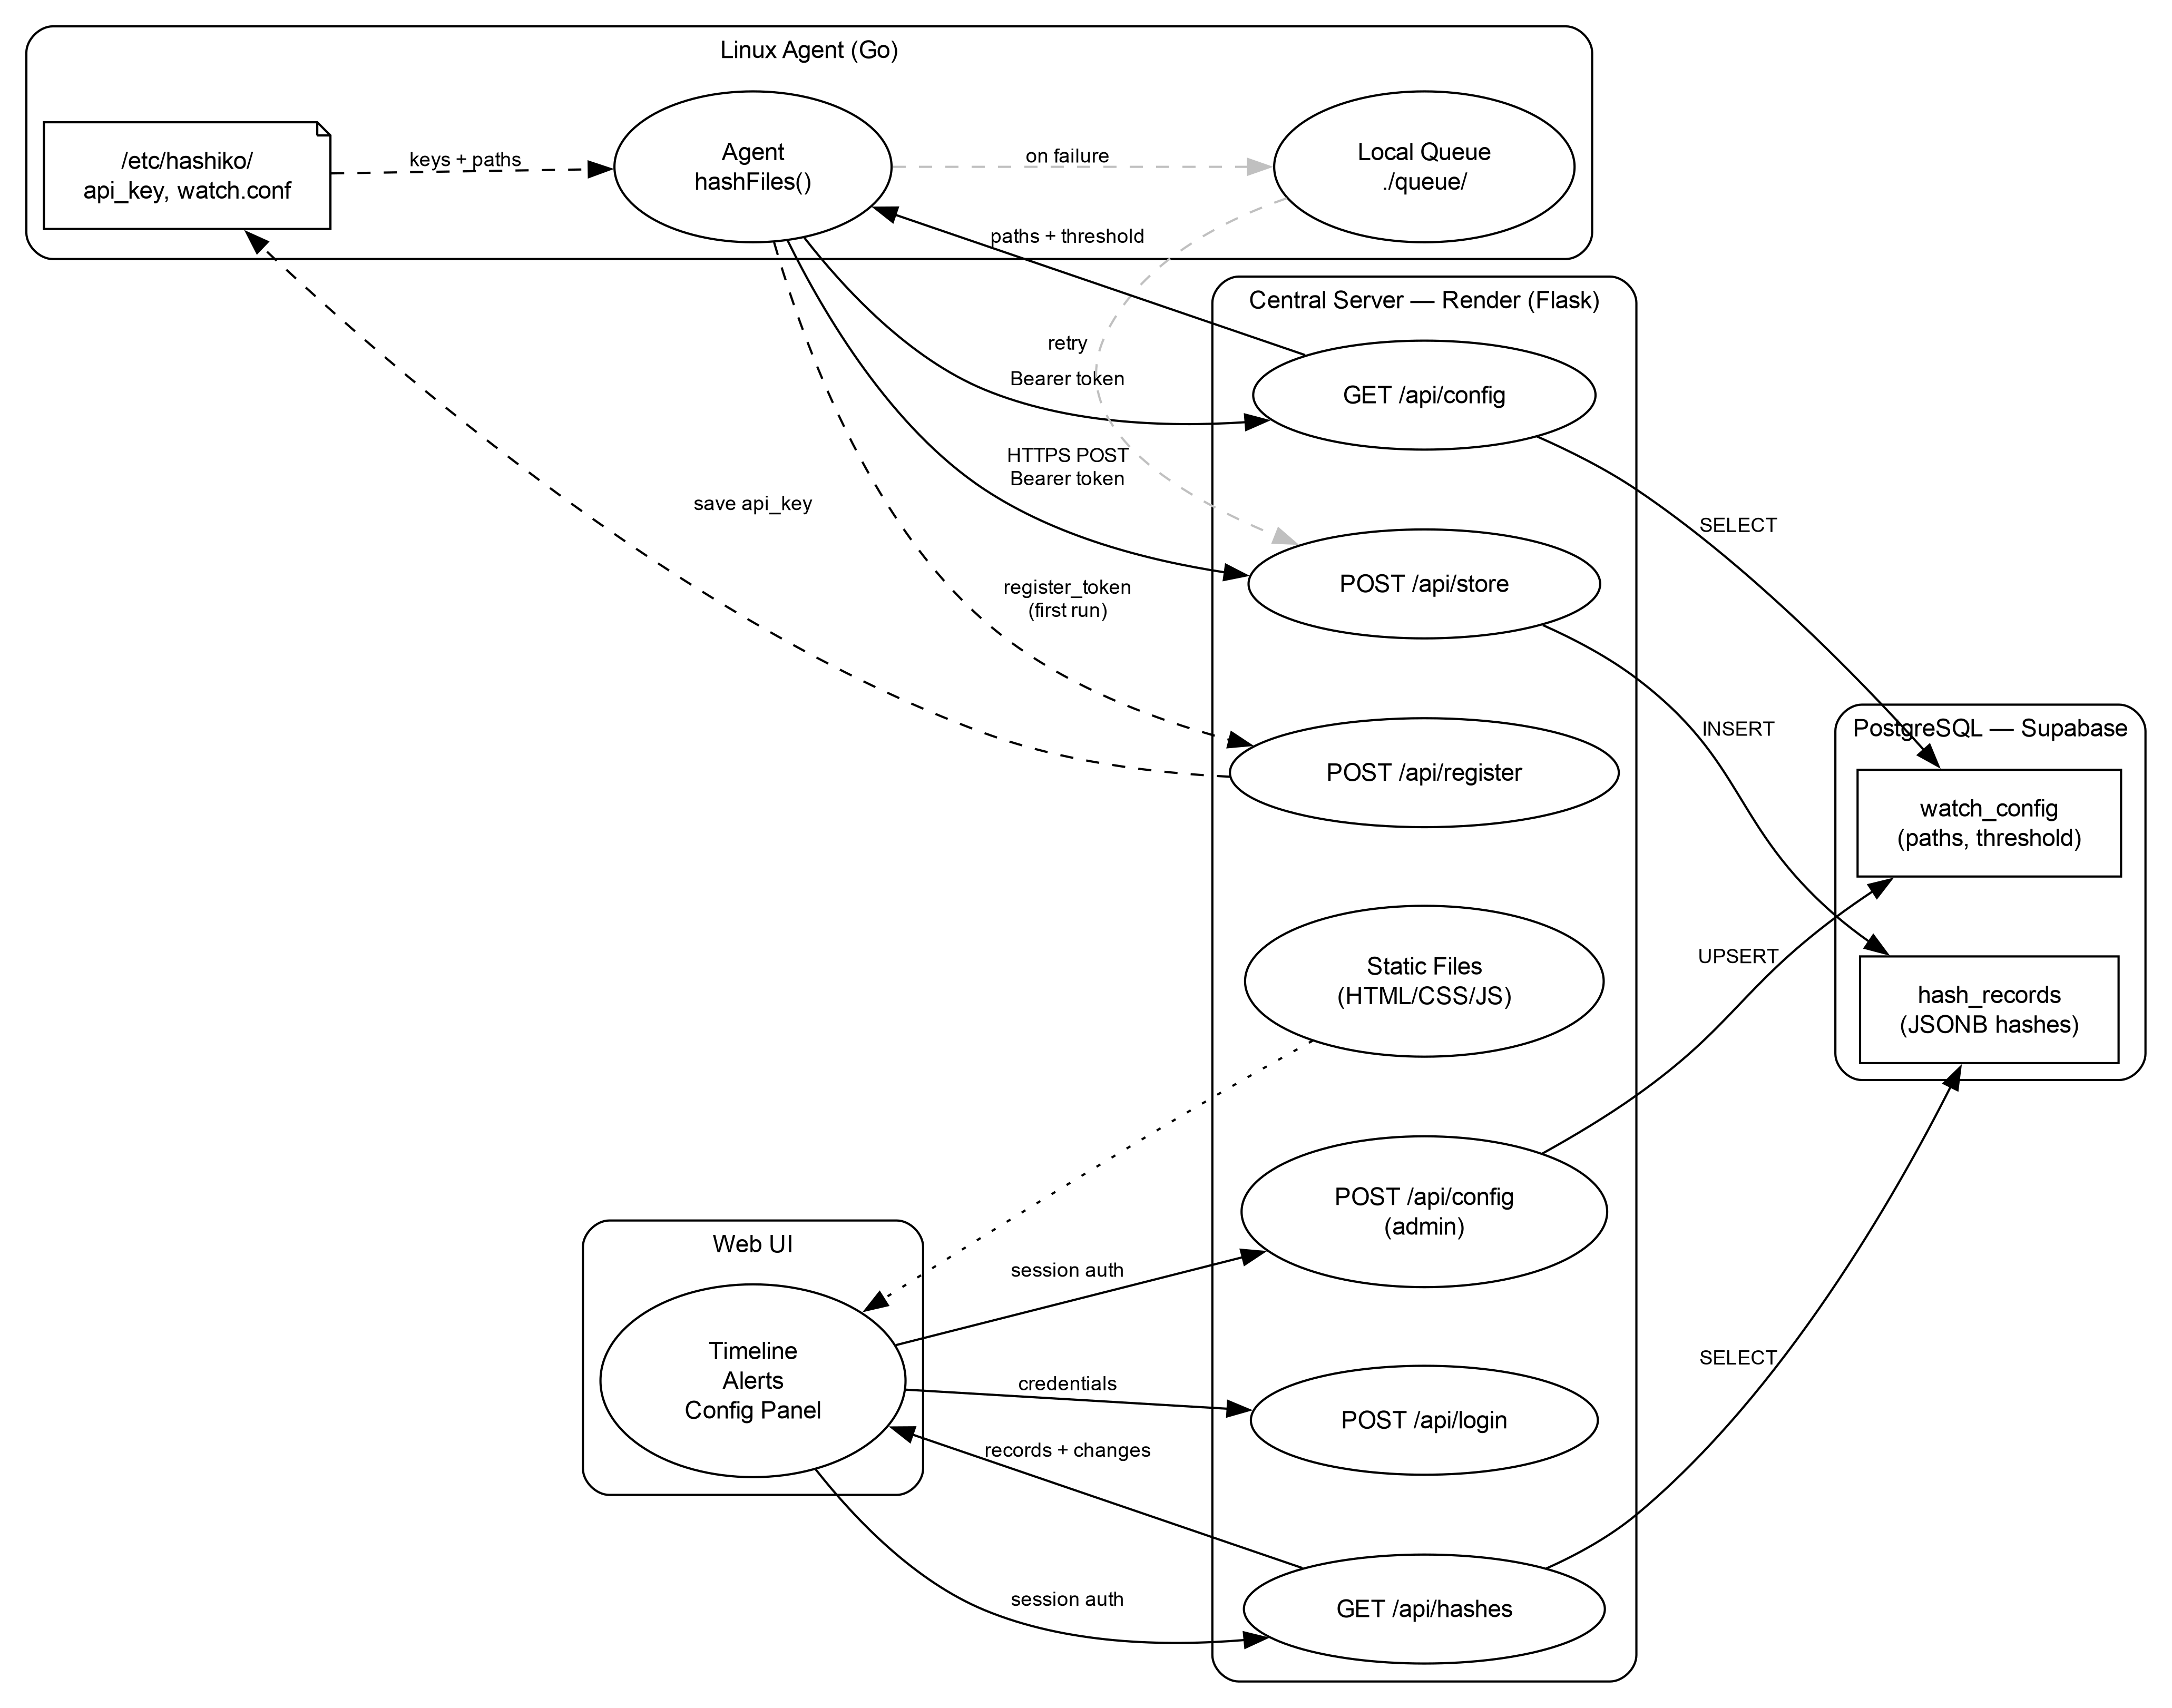
\includegraphics[width=\columnwidth]{../diagram/systems.png}
    \caption{System Architecture Diagram}
    \label{fig:systems}
\end{figure}

\subsection{Agent Architecture}

Figure \ref{fig:agent} shows the agent architecture. The agent uses SHA-256 hashing via \texttt{crypto/sha256}. SHA-256 is a cryptographic hash function that produces fixed-size output regardless of input length. This ensures that even a single bit change in a file generates a different hash value. The \texttt{hashFiles} function walks each monitored directory and computes an individual SHA-256 hash per file using \texttt{hashFile}. Files above the size threshold and volatile paths like .cache, .mozilla and tmp are skipped to reduce false positives and prevent performance issues. Each agent generates a unique ID from the username, hostname and \texttt{/etc/machine-id}. On first run, a registration token is exchanged for a persistent API key. Watch paths and the size threshold are fetched from the server on each run. JSON output includes timestamp, agent ID and a map of file paths to hashes. Transmission is via HTTPS POST to \texttt{/api/store}.

\begin{figure}[h!]
    \centering
    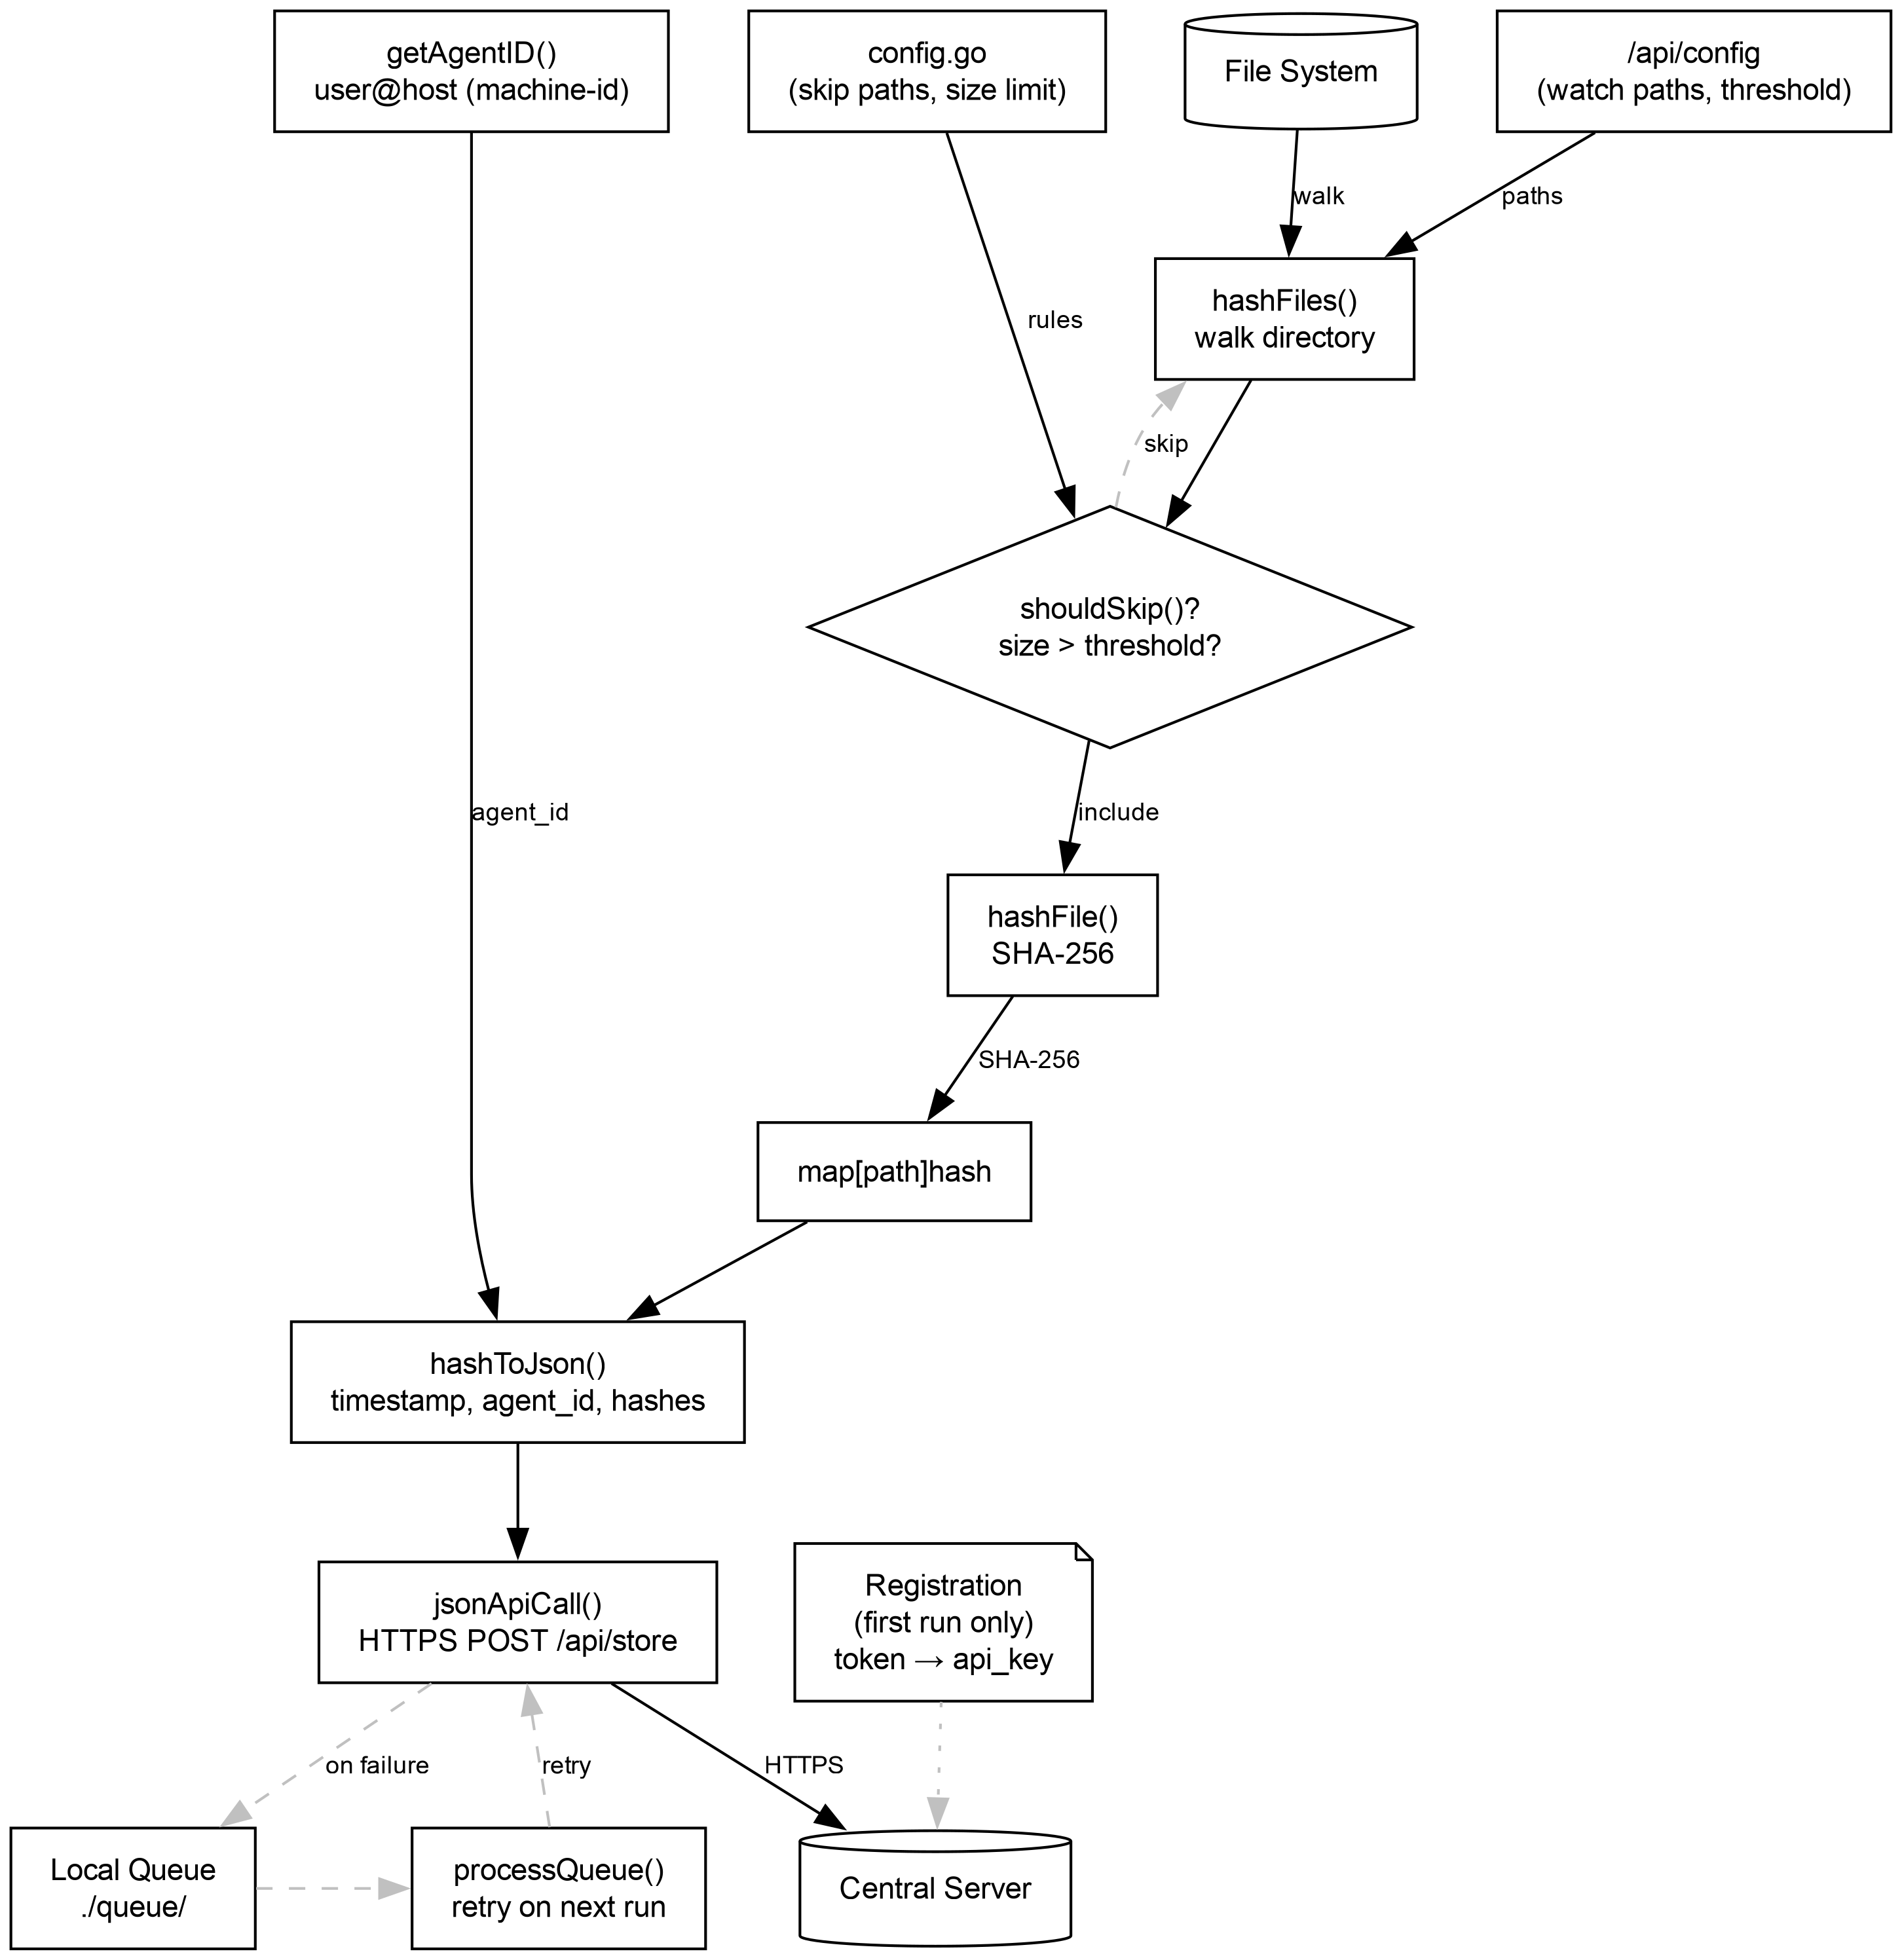
\includegraphics[width=\columnwidth]{../diagram/agent.png}
    \caption{Agent Architecture Diagram}
    \label{fig:agent}
\end{figure}

\subsection{Server Architecture}

Built with Flask and PostgreSQL. Loads environment variables and creates a \texttt{hash\_records} table with id, timestamp, agent\_id and a JSONB hashes column. A \texttt{watch\_config} table stores custom watch paths and the file size threshold per agent. The \texttt{/api/store} endpoint decodes JSON and inserts records with parameterized queries to prevent SQL injection. The \texttt{/api/hashes} endpoint returns all records with change detection applied. The \texttt{/api/config} endpoint serves watch paths and the threshold to agents. The \texttt{/api/register} endpoint handles one-time agent registration. Serves static files on port 8899. Deployed on Render with TLS provided automatically.

\subsection{Development}

Development followed an incremental approach. Milestone 1 implemented agent data collection, basic server storage, SHA-256 hashing and composite indexes. Milestone 2 added message queuing and retry logic. Milestone 3 added hash comparison, alerts and login. Milestone 4 added agent registration, per-agent configuration, security hardening and deployment. Milestone 5 added per-file hashing, a configurable file size threshold, automated tests and CI. Version control with Git enabled rollback if issues arose.

\subsection{Interface}

The HTML login page authenticates the admin via session-based auth. Once logged in, the agent grid shows all monitored machines with alert badges. Clicking an agent shows the hash timeline. Each row represents a report with a timestamp, file count and status badge. Rows with changes expand to show the exact files added, modified or deleted. A config panel allows the admin to set watch paths and the file size threshold per agent. An alert panel surfaces all changes detected in the last 24 hours.

\subsection{Database Schema}

Figure \ref{fig:database} shows the database schema diagram. The \texttt{hash\_records} table has an auto-incrementing id, TIMESTAMPTZ timestamp, TEXT agent\_id and a JSONB hashes column. The JSONB column stores a map of file path to SHA-256 hash string, supporting any number of monitored files without schema changes. A composite index on (timestamp, agent\_id) optimizes queries. The \texttt{watch\_config} table stores agent\_id, a JSONB array of custom paths and an integer file size threshold per agent.

\begin{figure}[h!]
    \centering
    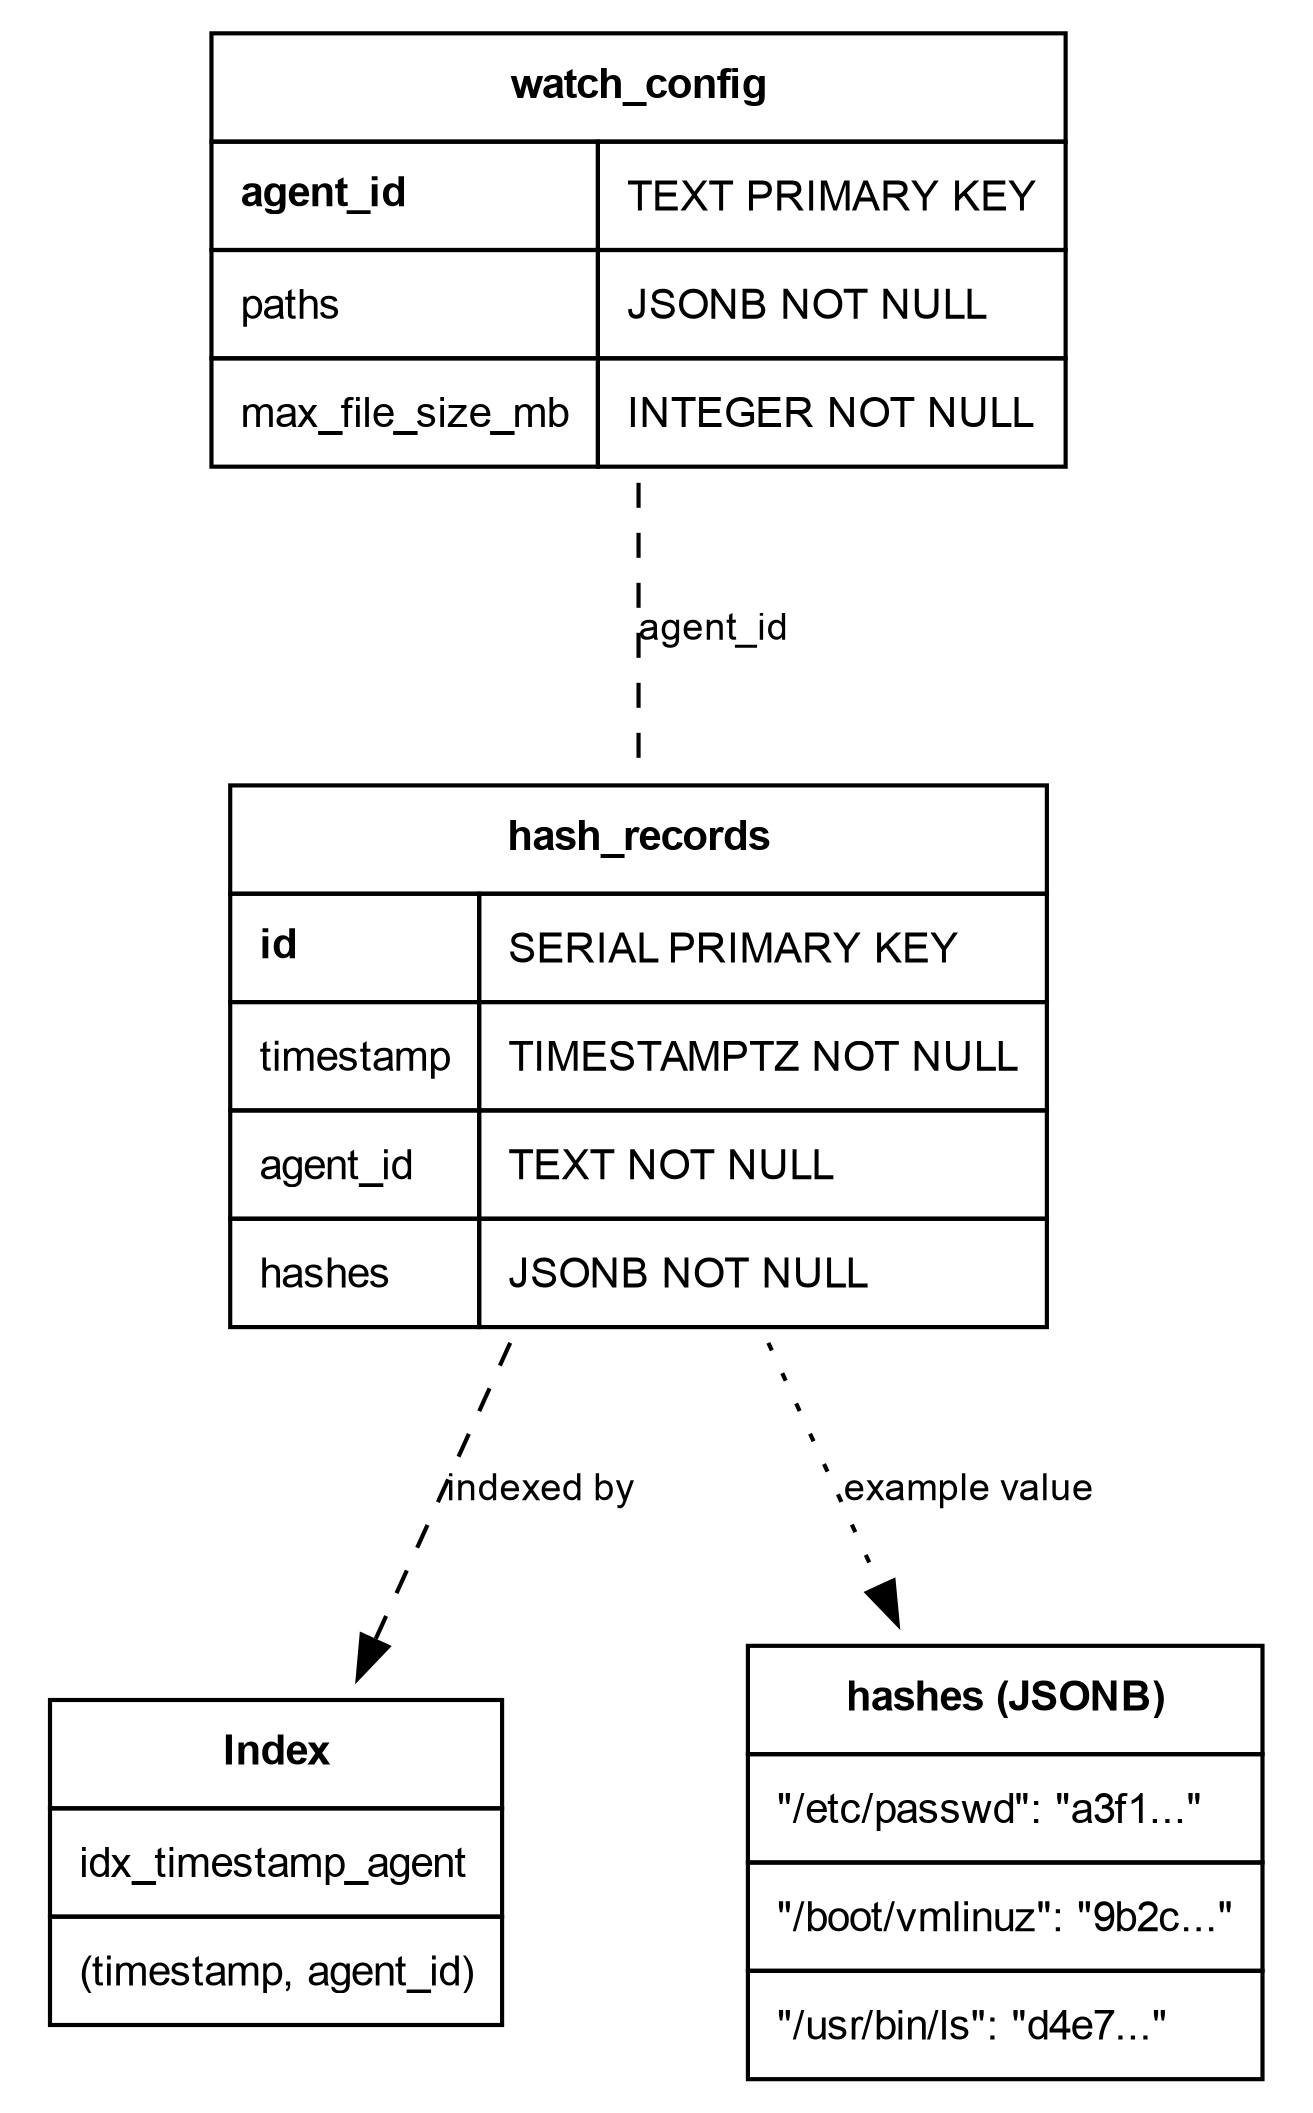
\includegraphics[width=\columnwidth]{../diagram/database.png}
    \caption{Database Schema Diagram}
    \label{fig:database}
\end{figure}

\subsection{Data Flow}

Figure~\ref{fig:sequence} shows the sequence of operations from agent registration through to the admin view. On first run, the agent exchanges a registration token for a persistent API key. It then fetches its watch paths and file size threshold from the server. On each subsequent run, the agent walks the monitored directories, computes a SHA-256 hash for each file and submits the report via HTTPS POST. If the server is unreachable, the report is saved to a local queue and retried on the next run. When the admin logs in, the web interface fetches all records from the server, applies change detection and displays the results in a timeline with alerts.

\begin{figure}[h!]
    \centering
    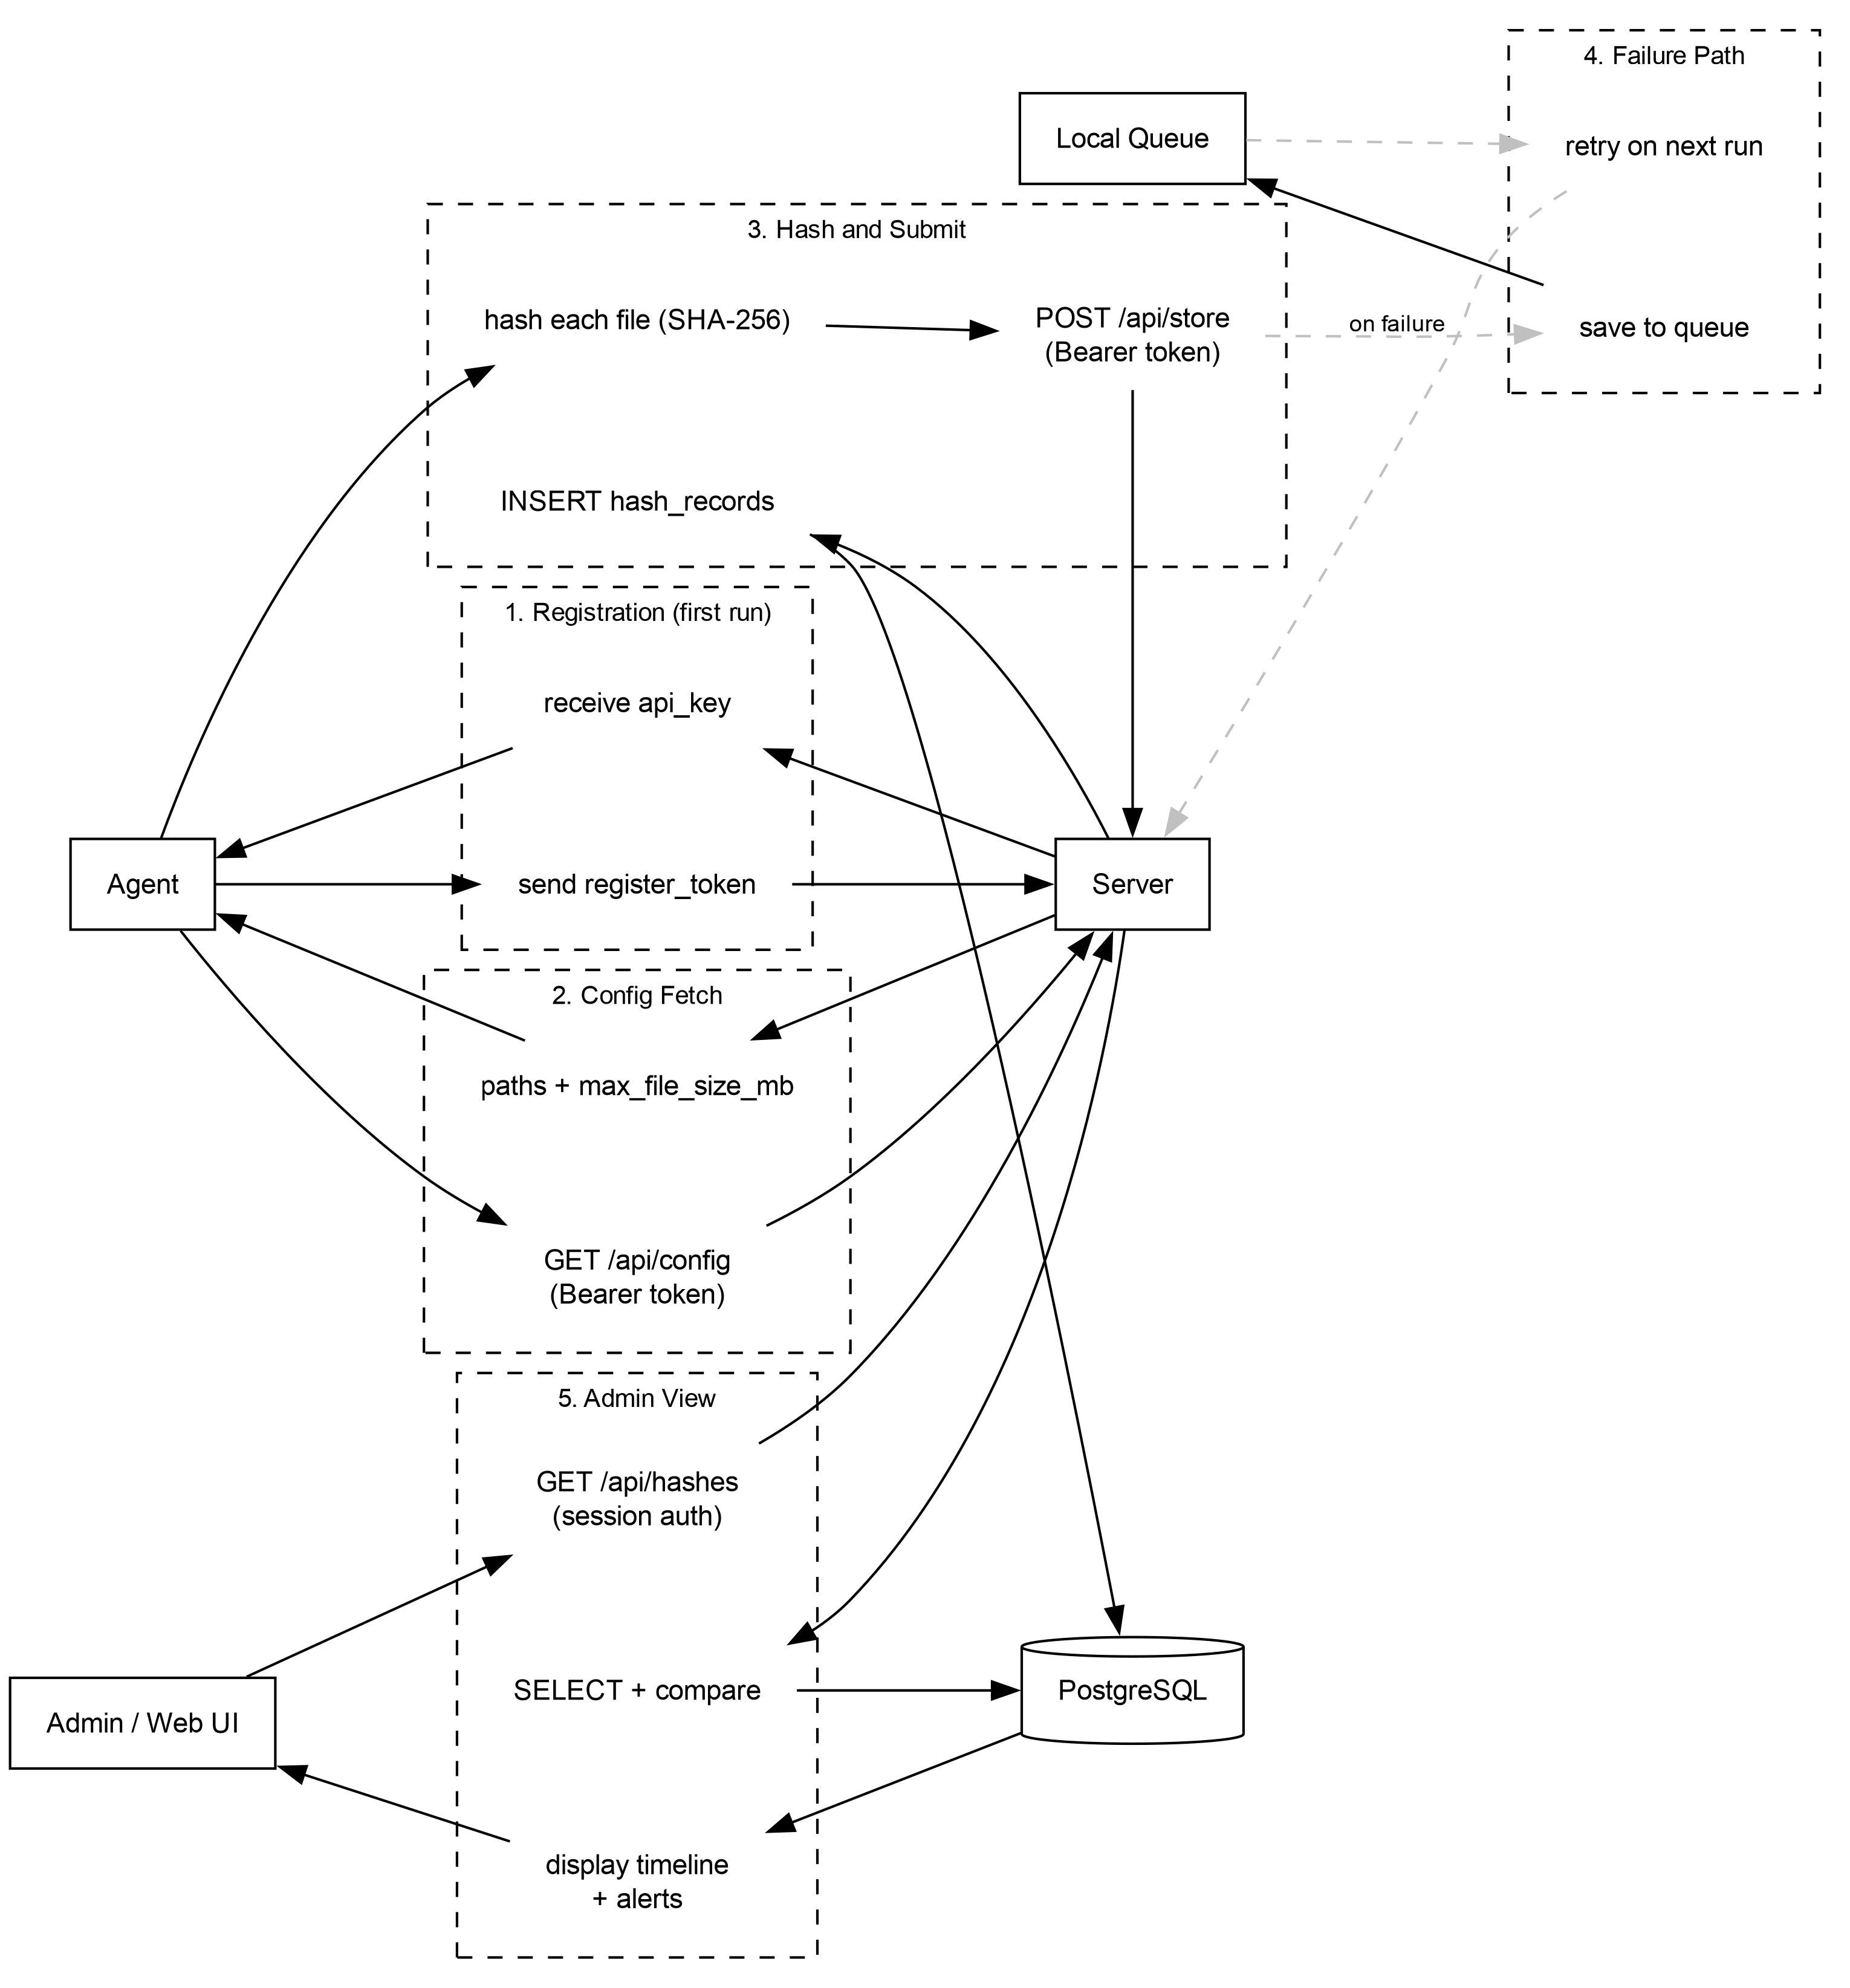
\includegraphics[width=\columnwidth]{../diagram/sequence.png}
    \caption{Data Flow Sequence Diagram}
    \label{fig:sequence}
\end{figure}

\section{Scope}

Scope includes agents, a central server, storage and a web interface. Features cover per-file integrity monitoring with SHA-256 hashes, timestamped reports, HTTPS-based transfer, queue-based retry logic, alerts, per-agent watch path configuration, file size threshold configuration and a timeline visualization. Deliverables are a Go agent, Flask server, PostgreSQL storage, web interface, documented APIs and a test suite with CI.

Out of scope are process monitoring, memory scanning, kernel exploit detection, malware analysis and compliance reporting. These exclusions distinguish Hashiko from comprehensive HIDS platforms like OSSEC. OSSEC includes rootkit detection and compliance reporting. Hashiko focuses on centralized per-file hash collection and storage.

\begin{table}[h]
\centering
\caption{In Scope vs Out of Scope}
\begin{tabular}{|p{4cm}|p{4cm}|}
\hline
\textbf{In Scope} & \textbf{Out of Scope} \\
\hline
Agents (Go), central server (Flask), PostgreSQL storage & Process monitoring / memory scanning \\
\hline
Per-file SHA-256 hashing, timestamped reports, HTTPS transfer & Kernel-level monitoring / rootkit detection \\
\hline
Alerts, login, timeline web interface & Compliance reporting / malware analysis \\
\hline
Per-agent watch path and file size threshold configuration & SIEM integration \\
\hline
Queue-based retry logic, documented APIs, test suite with CI & \\
\hline
\end{tabular}
\end{table}

\section{Technical Challenges}

\subsection{Agent Implementation Challenges}

Distributed agents must reliably collect and transmit data. Network interruptions must be handled without losing events. The queue system saves JSON hash data to local files when the server is unreachable. This prevents data loss during network interruptions. Successfully transmitted files must be removed to prevent duplicate submissions.

File hashing must be efficient. The agent walks large directory trees with potentially thousands of files. Volatile paths are filtered to reduce false positives. Large media files can cause the agent to hang or time out. A configurable file size threshold allows each agent to skip files above a set limit. This keeps the agent responsive on systems with large files such as media servers.

\subsection{Server and Storage Challenges}

The server must validate incoming data and prevent SQL injection. Parameterized queries are required for all database operations. Storage must support fast queries across multiple dimensions. A composite index on (timestamp, agent\_id) enables efficient filtering. The database must handle concurrent writes from multiple agents without data corruption.

\section{Testing and Results}

Hashiko includes automated tests for both the agent and the server. Tests run on every push through GitHub Actions CI. This ensures changes do not break existing behavior.

\subsection{Agent Tests}

The Go agent is tested using the built-in \texttt{testing} package. Nine unit tests cover hash computation accuracy, hash stability across runs, change detection, skip path filtering, large file exclusion and directory exclusion. A \texttt{clearSkips()} helper resets the global skip list before each test so temporary directory paths do not interfere.

\begin{table}[h]
\centering
\caption{Agent Unit Test Results}
\begin{tabular}{|p{4cm}|p{4cm}|}
\hline
\textbf{Test Case} & \textbf{Result} \\
\hline
Hash computation (SHA-256) & Pass \\
\hline
Hash stability across runs & Pass \\
\hline
Change detection & Pass \\
\hline
Skip path filtering & Pass \\
\hline
Large file exclusion & Pass \\
\hline
Directory exclusion & Pass \\
\hline
\end{tabular}
\end{table}

\subsection{Server Tests}

The Flask server is tested using pytest against a real PostgreSQL database. Twenty-three tests cover hash change detection, login, store, hashes retrieval, config GET and POST and agent registration. No mocking is used. Each test runs against a live database connection with a clean state enforced by a \texttt{clean\_db} fixture.

\begin{table}[h]
\centering
\caption{Server Test Coverage}
\begin{tabular}{|p{4cm}|p{4cm}|}
\hline
\textbf{Area} & \textbf{Tests} \\
\hline
Hash change detection & 6 \\
\hline
Login & 3 \\
\hline
Store (POST /api/store) & 4 \\
\hline
Hashes (GET /api/hashes) & 2 \\
\hline
Config GET and POST & 6 \\
\hline
Registration & 3 \\
\hline
\end{tabular}
\end{table}

\subsection{Continuous Integration}

GitHub Actions runs both test suites on every push. The agent job checks out the repository, sets up Go and runs \texttt{go test ./...}. The backend job starts a PostgreSQL service container, installs Python dependencies and runs \texttt{pytest}. Both jobs must pass before a merge is accepted.

\subsection{Test Environment}

Tests run on Fedora Linux with Python 3.14 and Go 1.24. The CI environment uses an Ubuntu runner with a PostgreSQL 15 service container. The backend uses \texttt{sslmode=disable} in CI and \texttt{sslmode=require} in production.

\section{Conclusion}

Hashiko implements centralized file integrity monitoring with distributed agents and queue-based retry logic. Each agent computes individual SHA-256 hashes for configurable watch paths and submits reports to a central server over HTTPS. All data is stored in a central PostgreSQL database with a composite index on timestamp and agent\_id for efficient querying. The web interface provides a timeline view of hash history, an alert panel and per-agent configuration.

The project addresses key limitations of traditional FIM tools. Centralized storage prevents local tool compromise. Queue-based retry ensures data durability during network interruptions. Alerts notify administrators when file changes are detected. The file size threshold prevents large files from blocking agent execution.

Future work could include automated change analysis and integration with SIEM platforms.

\begin{thebibliography}{00}
    \bibitem{kaczmarek} Kaczmarek, J. and Wrobel, M. (2008). Modern approaches to file system integrity checking. \textit{2008 1st International Conference on Information Technology}, 1--4. \url{https://doi.org/10.1109/inftech.2008.4621669}
    \bibitem{abdullah} Abdullah, Z. H., Udzir, N. I., Mahmod, R. and Samsudin, K. (2011). File integrity monitor scheduling based on file security level classification. \textit{Communications in Computer and Information Science}, 177--189. \url{https://doi.org/10.1007/978-3-642-22191-0_16}
\end{thebibliography}

\end{document}
